%%quellen
%% http://www.raspbian.org/RaspbianDocumentation
%% http://www.raspberrypiguide.de
%% http://www.raspberrypi.org
%%
%% Beuth Hochschule für Technik --  
%%
%% Kapitel 2 - Raspberry Pi
%%
%%	
\chapter{Raspberry Pi}

Das Raspberry Pi ist ein kreditkartengroßer Einplatinencomputer von der \textit{Raspberry Pi Foundation}\footnote{Stiftung und Wohltätigkeitsorganisation in Großbritannien} entwickelt wurde. Mithilfe seiner 700 MHz starken ARM-CPU kann er nahezu alles was auch normale Desktoprechner können.\\
Ziel der Entwicklung des Raspberry Pi ist das Interesse an dem Studium der Informatik und ähnliche Fachgebiete zu fordern, bwz. einen günstigen Computer zum Programmieren und Experimentieren anbieten zu können.\\

Durch die geringe Leistungsaufnahme, günstigen Preis und viele verschiedene Ausbau- und Personalisierungsmöglichkeiten können Raspberry Pi’s für verschiedene Zwecke eingesetzt werden. Unter anderem sind beliebte Projekte für den Haushalt Wetterstationen, Radiosender, Media Center, NAS, etc.



%%%%%%%%%%%%%%%%%%%%%%%%%%%%%%%%%%%%%%%%%%%%%%%%%%%%%%%%%%%%%%%%%%%%%%
\section{Hardware}
%%-------------------------------------------------------------------
\subsection{Technische Spezifikationen}

\begin{figure}[h]
  \begin{center}		%width=\linewidth
    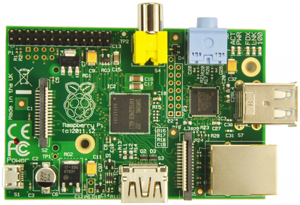
\includegraphics[scale=0.4]{raspberrypi-model-b.png}
  		  \caption{Raspberry Pi Model B}
     \label{raspPic}
  \end{center}
\end{figure}

\begin{longtable}{||l|l||}

\hline
Testfall & Fehler\\ \hline\hline
\endfirsthead
\hline
Testfall & Fehler & Kommentar & Errorcode \\ \hline\hline
\endhead

Größe & 85,60 x 53,98 x 17 mm\\ \hline
Soc & Broadcom BCM2835\\ \hline
CPU & ARM1176JZF-S(700MHz)\\ \hline
GPU & Broadcom VideoCore IV \\ \hline
SDRAM & 512MB
USB 2.0 & 2\\ \hline
Videoausgabe & HDMI \& S-Video\\ \hline
Tonausgabe & 3,5mm Klinkenstecker \& HDMI\\ \hline
Speicher & SD(SDHC/SDXC)/MMC/SDIO Kartenleser bis 128GB\\ \hline
Netzwerk & 10/100 MBit Ethernet\\ \hline
Schnittstellen & 17 GPIO-Pins, SPI, 21C, UART\\ \hline
Stromversorgung & 5V Micro-USB Anschluss\\ \hline

\end{longtable}
\footnote{http://www.raspberrypiguide.de; http://www.raspberrypi.org; 15.01.2014}

%%-------------------------------------------------------------------
\subsection{Kamera}

\begin{figure}[h]
  \begin{center}		%width=\linewidth
    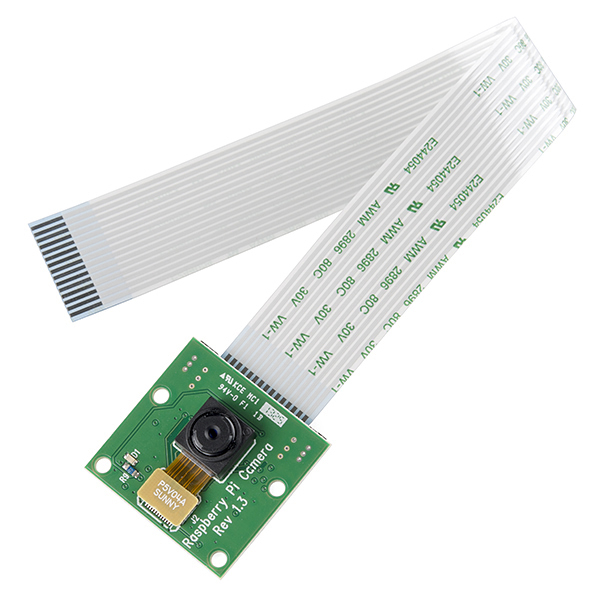
\includegraphics[scale=0.3]{camera.jpg}
  		  \caption{Raspberry Kamera}
     \label{raspCam}
  \end{center}
\end{figure}


\begin{longtable}{||l|l||}

\hline
Testfall & Fehler\\ \hline\hline
\endfirsthead
\hline
Testfall & Fehler & Kommentar & Errorcode \\ \hline\hline
\endhead

Größe & 20 x 24 mm\\ \hline
Sensor & OmniVision OV5647 (5MP)\\ \hline
Auflösung & 2592 x 1944\\ \hline
Video & 1080p \@ 30fps \\ \hline
SDRAM & 512MB
Anschluss & 15-Pin Flachbandkabel\\ \hline

\end{longtable}


%%%%%%%%%%%%%%%%%%%%%%%%%%%%%%%%%%%%%%%%%%%%%%%%%%%%%%%%%%%%%%%%%%%%%%
\section{Software und Einstellungen}

%%-------------------------------------------------------------------
\subsection{Betriebssystem}
Für das Raspberry Pi worden mehrere Open Source Betriebssysteme programmiert. Alle basieren auf verschiedene Linux Distributionen(u.a. OpenSUSE, Fedora, FreeBSD, Debian). Je nach Bedarf kann sich jeder Nutzer für eine Distribution entscheidend, eins des beliebtestens Raspbian, basierend auf Debian, was auch in diesem Projekt benutzt wird. Raspbian inkludiert alle Grundprogramme und -Utilities dass mit vielen verschiedenen Packages kompatibel sind. Dieser Betriebssystem hat sich im laufe der Zeit als sehr stabil bewiesen.\\

Es gibt auch die Möglichkeit Windows auf das Raspberry Pi zu installieren, obwohl Nutzer davon abgeraten werden. Das Windows Betriebssystem benötigt zu viele Ressourcen und läuft sehr langsam und instabil auf das Raspberry Pi.\\

Andere Distributionen sind Gebrauchorientiert aufgestellt, wie zum Beispiel für Media Center das beliebte XBMC (OpenELEC, Raspbmc, XBian). Weiterhin gibt es auch Androidsysteme die auf das Raspberry Pi portiert worden sind.
\footnote{http://www.raspbian.org; 15.01.2014}


%%-------------------------------------------------------------------
\subsection{LAMP Webserver}
LAMP steht für Linux Apache MySQL PHP Webserver. Auf das Raspberry Pi wurde ein LAMP Server installiert um die Desktop/Mobil Applikation mit dem Pi zu verbinden und Informationen Austauschen. Durch die Einstellung eines DNS kann auf das Videostreams sowie auf die MySQL Datenbank zugegriffen werden. Damit \textit{http} oder \textit{ssh} Anfragen  an das Server im Raspberry Pi ankommen, müssen Ports für die Verbindung zur Verfügung gestellt werden. Im diesen Fall muss jeweils ein Port für die SSH-Verbindung, den Videostream und die Datenbankzugriffe freigegeben werden.\\

Um das LAMP Webserver zu installieren werden folgende Kommandos mit Administratorrechte ausgeführt:\\
\begin{lstlisting}
apt-get install apache2
apt-get install mysql-server
sudo apt-get install php5
sudo apt-get install php5-mysql
\end{lstlisting}

%%-------------------------------------------------------------------
\subsection{SSH Zugriff}
Damit das Team gleichzeitig auf das Raspberry Pi arbeiten konnte wurde auf das System eine SSH-Verbindung eingestellt. So wurden auch Entwicklungskosten gesparrt, weil nicht jeder Teammitgleid ein System benötigte.\\
Um das Raspberry Pi per Fernzugriff zu betreiben ist es nötig eine \textit{Secure Shell} Verbindung aufzubauen. Aus Sicherheitsgründen wurde der Standardport für SSH-Verbindungen (Port 22) auf ein anderes geändert. Durch die Verfügung einer SSH-Verbindung können Updates, Support und Wartungsarbeiten per Fernzugriff auf das System ausgeübt werden, dieses sparrt kosten für den Kunden sowie für den Support.


%%-------------------------------------------------------------------
\subsection{DNS}
Um das Raspberry Pi über das lokale Netz erreichbar zu machen, wurde erstmal ein Webserver aufgebaut. Um jetzt das System überall über das Internet erreichbar ist, muss eine Domain reserviert werden. Somit kann ein Benutzer zugriffe auf die Datenbank sowie auf das Videostream aus jedem Rechner oder Android Mobilgerät weltweit ausüben. Der Dienst \”no ip\” bietet solche Dienstleistung kostenlos an. Für dieses Projekt wurde die Adresse \textit{spyhole.no-ip.biz) eingestellt und durch die Freigabe und Weiterleitung von Ports können die programmierten Applikationen auf das Raspberry Pi zugreifen.\\

%%-------------------------------------------------------------------
\subsection{…}

%%%%%%%%%%%%%%%%%%%%%%%%%%%%%%%%%%%%%%%%%%%%%%%%%%%%%%%%%%%%%%%%%%%%%%
\section{OpenVC}

%%-------------------------------------------------------------------
\subsection{Gesichtserkennung}


%%%%%%%%%%%%%%%%%%%%%%%%%%%%%%%%%%%%%%%%%%%%%%%%%%%%%%%%%%%%%%%%%%%%%%
\section{MJPG Streamer}

%%-------------------------------------------------------------------
\subsection{subsection}